\documentclass[a4paper,12pt]{report}

\usepackage{alltt, fancyvrb, url}
\usepackage{graphicx}
\usepackage[utf8]{inputenc}
\usepackage{float}
\usepackage{xcolor}
\usepackage{hyperref}

% Questo commentalo se vuoi scrivere in inglese.
\usepackage[italian]{babel}

\usepackage[italian]{cleveref}

\title{``L'Armata delle Tenebre''}

\author{Fabrizio Marzo}
\date{Luglio 2025}


\begin{document}%Questo specifica l'inizio del Documento

\maketitle

\tableofcontents % Il comando genera automaticamente l’indice (cioè la tabella dei contenuti) del documento, in base a tutte le sezioni, sottosezioni, capitoli, ecc. che hai usato con i comandi \chapet, \section, \subsection, ecc.

\chapter{Analisi} % Definisco il primo Capitolo.

% Questo è come fare commenti in latex, con il simbolo '%'.
% \textit{testo}, definisco quello che voglio scrivere in corsivo.
% \textbf{testo}, definisco quello che voglio scrivere in grassetto.
% \emph{testo}, definisco del testo che voglio mettere in evidenza.
% \begin{itemize} (Dico dove inizia le sezione con i pallini) \item (Indico un pallino) \end{itemize} (Dico dove finisce la sezione con i pallini).
% \chapter{nome capitolo}, Indico un capitolo e il nome del capitolo.
% \section{nome sezione capitolo}, Indico una sezione del capitolo, con il suo nome.
%\subsection{nome sotto-sezione}, Indico una sotto-sezione di una sezione.

\section{Requisiti}

L'applicazione emula il gioco 2D per smartphone \emph{Survivor.io}, con alcune modifiche alla gestione del personaggio (il \emph{Survivor}) e al comportamento dei nemici (gli \emph{Zombie}). L'obiettivo del gioco è far sopravvivere il Survivor a tutte le ondate di Zombie previste per il livello.

\begin{itemize}
    \item \textbf{Inizio partita:} Il Survivor inizia la partita in una posizione predefinita, già equipaggiato con un’arma (una \emph{pistola}). Gli Zombie entrano nel livello da posizioni casuali, che possono trovarsi sia all’interno che all’esterno dei confini della mappa, e iniziano immediatamente a inseguire il Survivor.

    \item \textbf{Fase di combattimento:} Il Survivor deve evitare gli Zombie spostandosi liberamente all’interno dei limiti del livello (\textbf{non} oltre). Può sparare in tutte le direzioni con l’arma equipaggiata. I colpi sono infiniti, grazie a un meccanismo di \emph{ricarica automatica}.

    \item \textbf{Fine partita:} La partita termina quando il Survivor riesce a sopravvivere a tutte le ondate zombie stabilite per il livello, eliminando tutti gli Zombie presenti.
\end{itemize}


\subsection*{Requisiti Funzionali}
\begin{itemize}
	\item Il gioco deve gestire correttamente il movimento degli Zombie verso il target (Survivor), evitando la sovrapposizione tra di essi durante il movimento e rallentandone la velocità quando si trovano vicini ad altri Zombie.
	
	\item Il gioco deve gestire correttamente la meccanica di sparo del Survivor verso gli Zombie, includendo una gestione precisa delle collisioni tra munizioni e Zombie, oltre al movimento del Survivor all'interno dei limiti della mappa di gioco.
	
	\item La gestione del livello è affidata a un \texttt{LevelManager}, responsabile della creazione delle ondate di Zombie in base a intervalli di tempo prestabiliti.
	
	\item Deve essere rispettata una chiara separazione tra la parte di \textit{View} e quella di \textit{Model}, in linea con l'architettura MVC.
\end{itemize}

\section{Analisi e Modello del Dominio}

Il progetto si pone l'obiettivo di separare il dominio logico del gioco dalla parte grafica, seguendo il principio dell'architettura MVC.

La parte di \textbf{Model} (dominio) contiene le principali \emph{entità} del gioco, come i diversi tipi di \emph{Survivor}, \emph{Zombie} e \emph{Livelli}. Ogni entità è caratterizzata da dimensioni specifiche espresse in \textbf{centimetri} (\textbf{unità di misura del modello}).
%
Essendo un gioco in 2D, si è scelto di non creare una classe dedicata \texttt{Vettore2D}, ma di utilizzare la classe \texttt{Pair} di Apache. Entrambe le soluzioni sono molto simili sia nell’implementazione sia nell’utilizzo all’interno del progetto, e la classe \texttt{Pair} incapsula esattamente l’informazione desiderata, ovvero una coppia di valori.
%
Il progetto distingue chiaramente tra le entità del modello e le entità di gioco. Le entità di gioco sono composte dalla parte grafica e dall’entità di riferimento; per i Survivor è inclusa anche la componente di input.

Questa “traduzione” avviene durante l’avvio del gioco: il livello del modello viene convertito in un livello di gioco e, a cascata, tutti gli Zombie e i Survivor vengono trasformati da entità di modello in entità di gioco.

\begin{center}
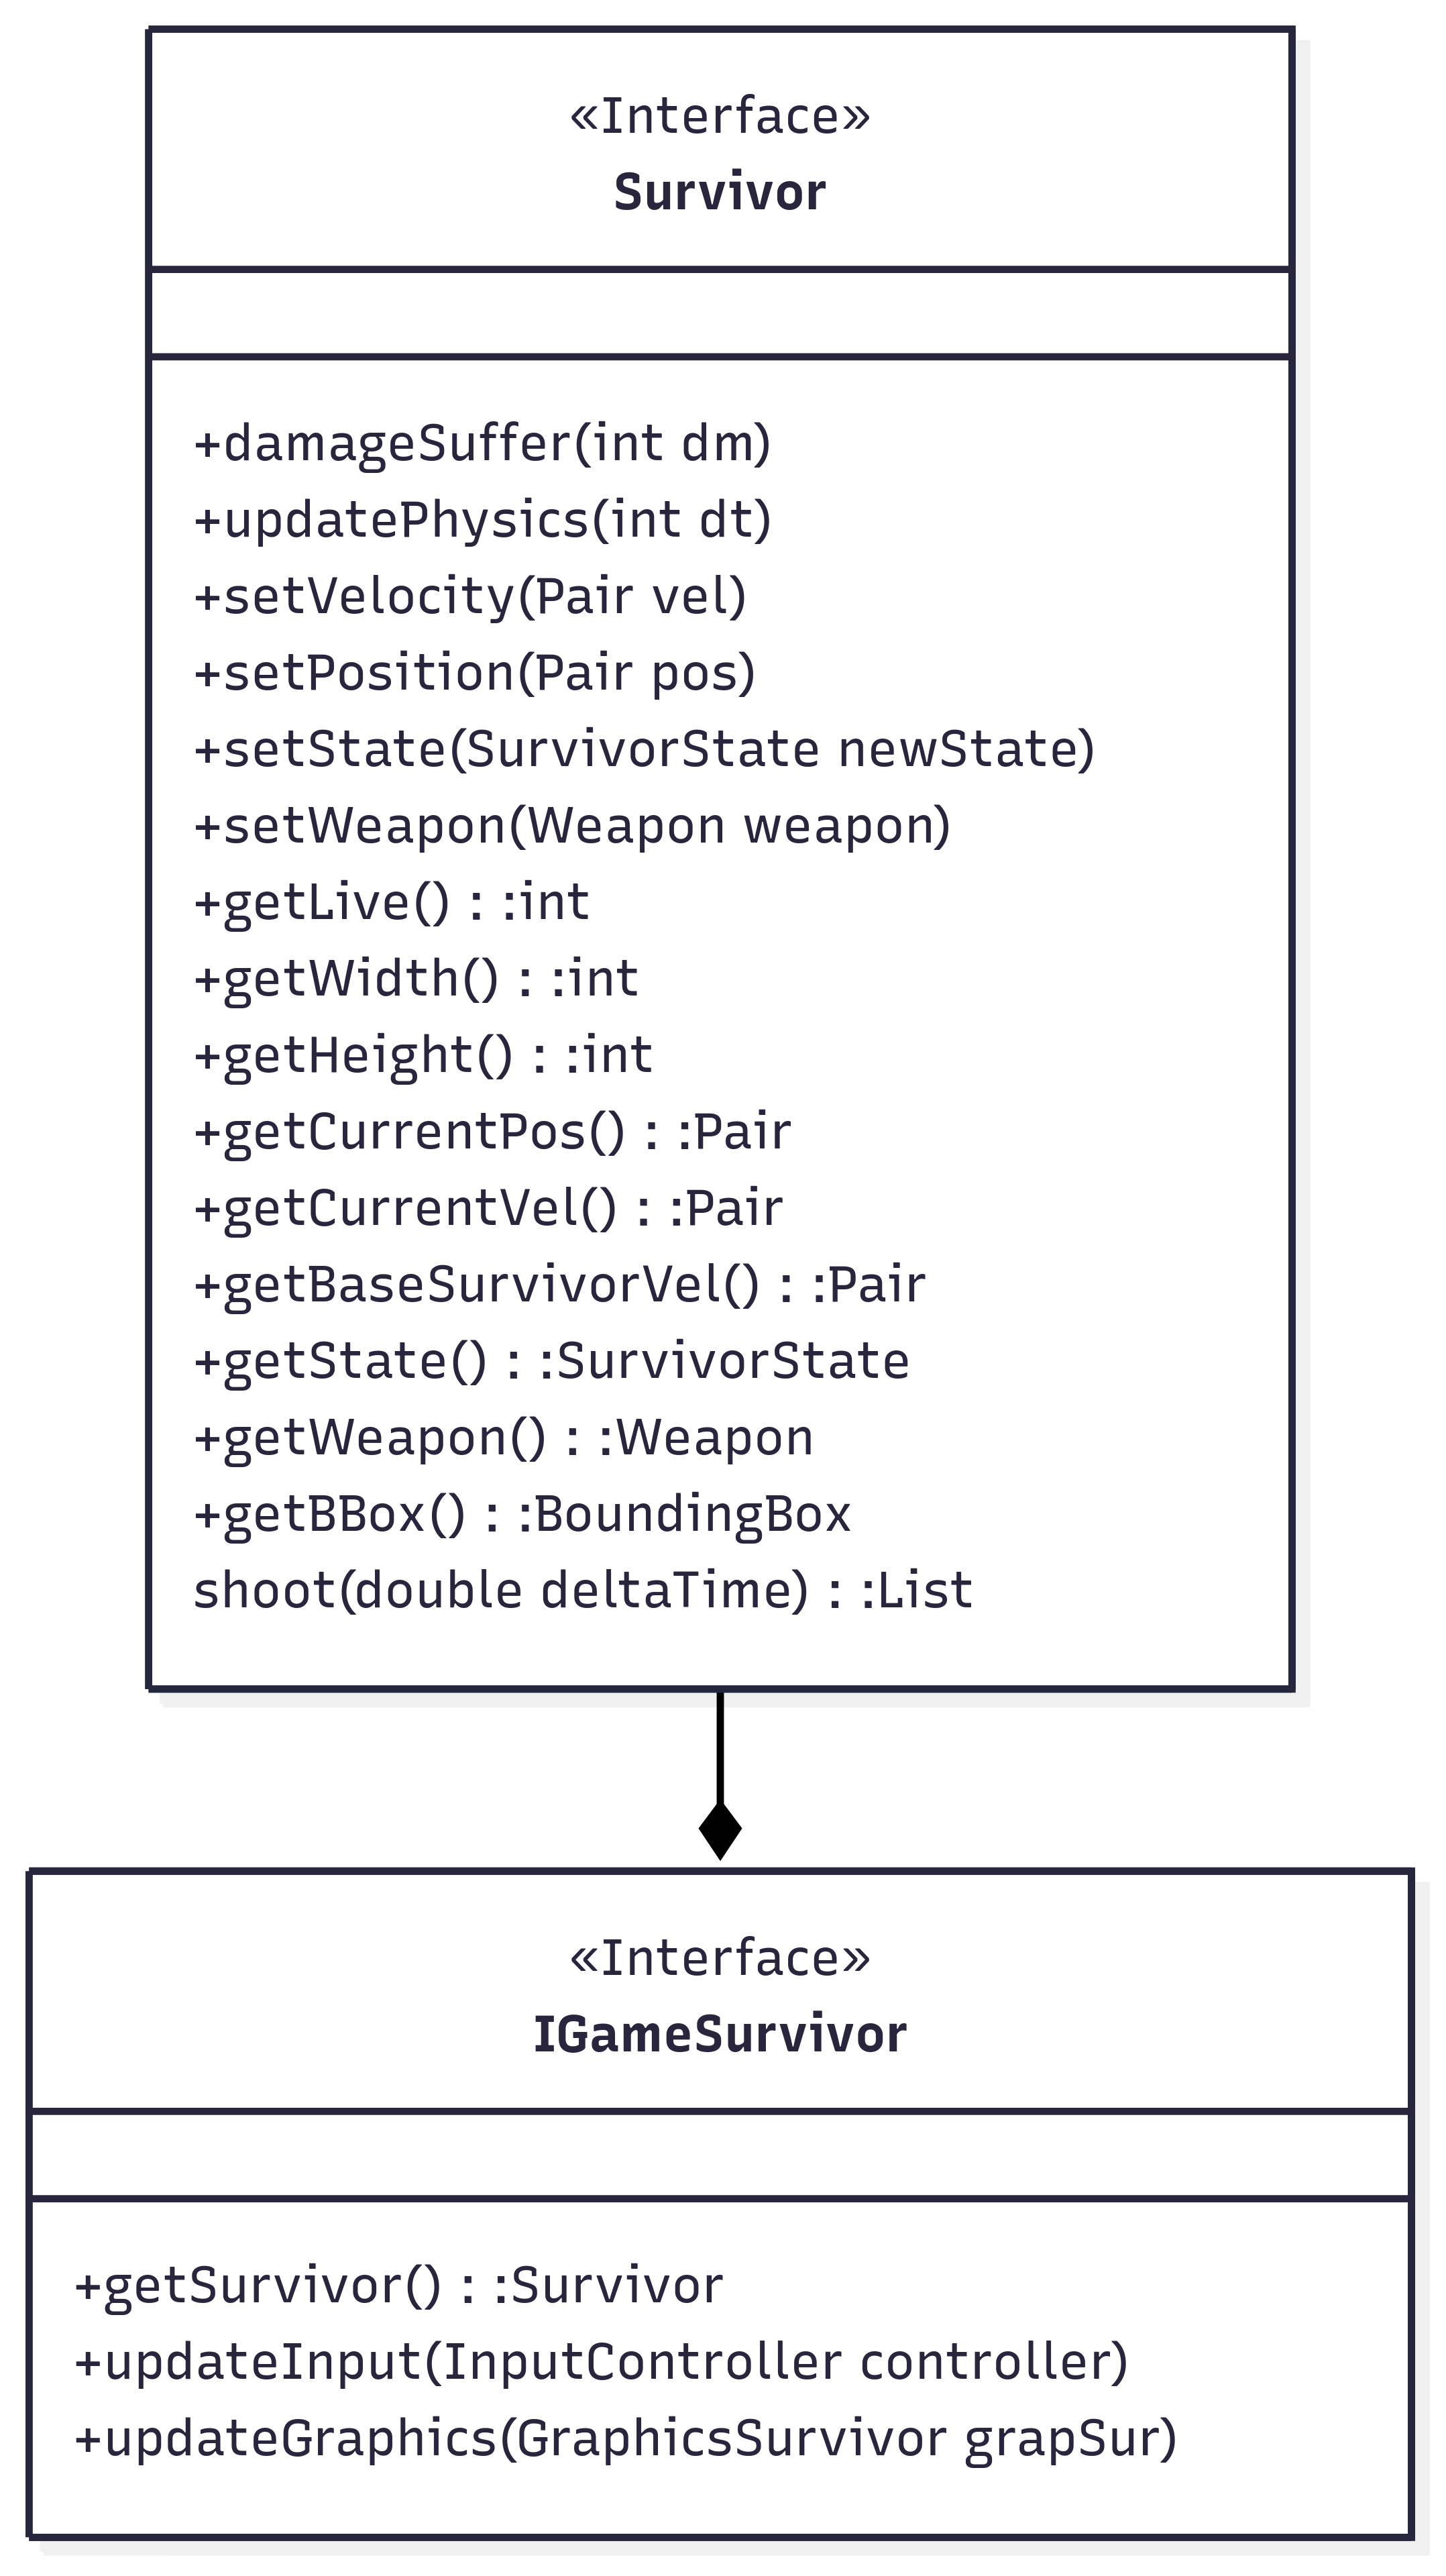
\includegraphics[width=0.5\textwidth]{img/Survivor-SurvivorGame.png}
\end{center}
Schema UML, rappresenta l'Entità di gioco Survivor.

\chapter{Design}

\section{Architettura}
\section{Implementazione del Pattern MVC e uso del Pattern Composite}
%
L'idea fondamentale alla base del mio progetto, in linea con il paradigma MVC (Model-View-Controller), è la seguente: nel \texttt{package \textbf{model}} definisco tutte le entità che rappresentano ciò che il mio mondo, in altre parole, qui risiedono le classi che descrivono gli oggetti di gioco a livello concettuale e logico, come il \texttt{Survivor}, gli \texttt{Zombie}, i \texttt{Livelli} e l'\texttt{Armamentario}.
%
Nel \texttt{package \textbf{game}} invece si trova il vero e proprio “mondo di gioco”, ovvero la rappresentazione attiva e interattiva di questi elementi durante l'esecuzione del gioco. Qui gli elementi del \texttt{model} vengono trasformati in oggetti giocabili e dinamici.
%
Per realizzare questa trasformazione, ed implementare efficacemente il pattern MVC, ho fatto uso del \textbf{pattern Composite}. Questo perché gli elementi di gioco non sono semplici oggetti isolati, ma sono \textit{composti} da più componenti:
%
\begin{itemize}
    \item una \textbf{componente grafica} comune a tutti gli elementi, necessaria per la loro rappresentazione visiva sullo schermo;
    \item in alcuni casi, come per il \texttt{Survivor}, anche una \textbf{componente di input} che permette di gestire l'interazione diretta con il giocatore.
\end{itemize}

Questa composizione consente di costruire un’entità di gioco che integra in modo modulare sia la logica interna (definita nel \texttt{model}) sia la sua rappresentazione e la sua interattività (gestite nel \texttt{game}).

In sintesi, per implementare il pattern MVC nel mio progetto, ho dovuto necessariamente adottare il pattern Composite: grazie a questo, ogni elemento di gioco è strutturato come un oggetto composto da più sotto-elementi (componenti grafiche, input, ecc.), permettendo una chiara separazione tra modello, vista e controllo e facilitando la gestione di oggetti complessi nel contesto di gioco.
%%%%%%%%%%%
\section{Ulteriore Utilizzo del Pattern Composite e Introduzione del Pattern Factory}

Un ulteriore aspetto importante dell’uso del pattern Composite nel mio progetto riguarda la flessibilità e la variabilità delle componenti che costituiscono gli elementi di gioco. In particolare, tutte le componenti che vengono utilizzate all’interno delle classi nel \texttt{package game} possono variare, sia in fase di creazione degli oggetti di gioco sia durante il loro ciclo di vita.

Ad esempio, per la componente grafica e per la gestione dell’input non è detto che si debbano usare sempre le stesse implementazioni. A seconda delle esigenze o delle configurazioni, è possibile adottare diverse varianti per rappresentare e controllare un’entità come il \texttt{GameSurvivor}.

Per gestire questa variabilità ho fatto uso del \textbf{pattern Factory}, che permette di creare oggetti con diverse implementazioni senza modificare il codice client che li utilizza. In pratica, la Factory incapsula la logica di creazione degli oggetti, restituendo l’istanza più adatta in base al contesto o ai parametri forniti.

Nel mio progetto, la Factory viene utilizzata in due ambiti principali:

\begin{itemize}
    \item nella creazione degli oggetti di gioco all’interno del \texttt{package game}, ad esempio per istanziare un \texttt{GameSurvivor}, \texttt{GameZombie}, \texttt{GameLevel}, con una determinata componente grafica o con una diversa gestione dell’input, a seconda delle specifiche esigenze;
    \item anche nella parte di \texttt{model}, per la creazione delle entità di base come \texttt{Survivor}, \texttt{Zombie}, \texttt{Level}, garantendo un metodo centralizzato e flessibile per l’istanziazione degli oggetti modello.
\end{itemize}

Questa combinazione di pattern Composite e Factory consente di ottenere un’architettura estremamente modulare, estendibile e facilmente mantenibile, capace di adattarsi a nuove necessità senza richiedere modifiche invasive al codice esistente.


\begin{center}
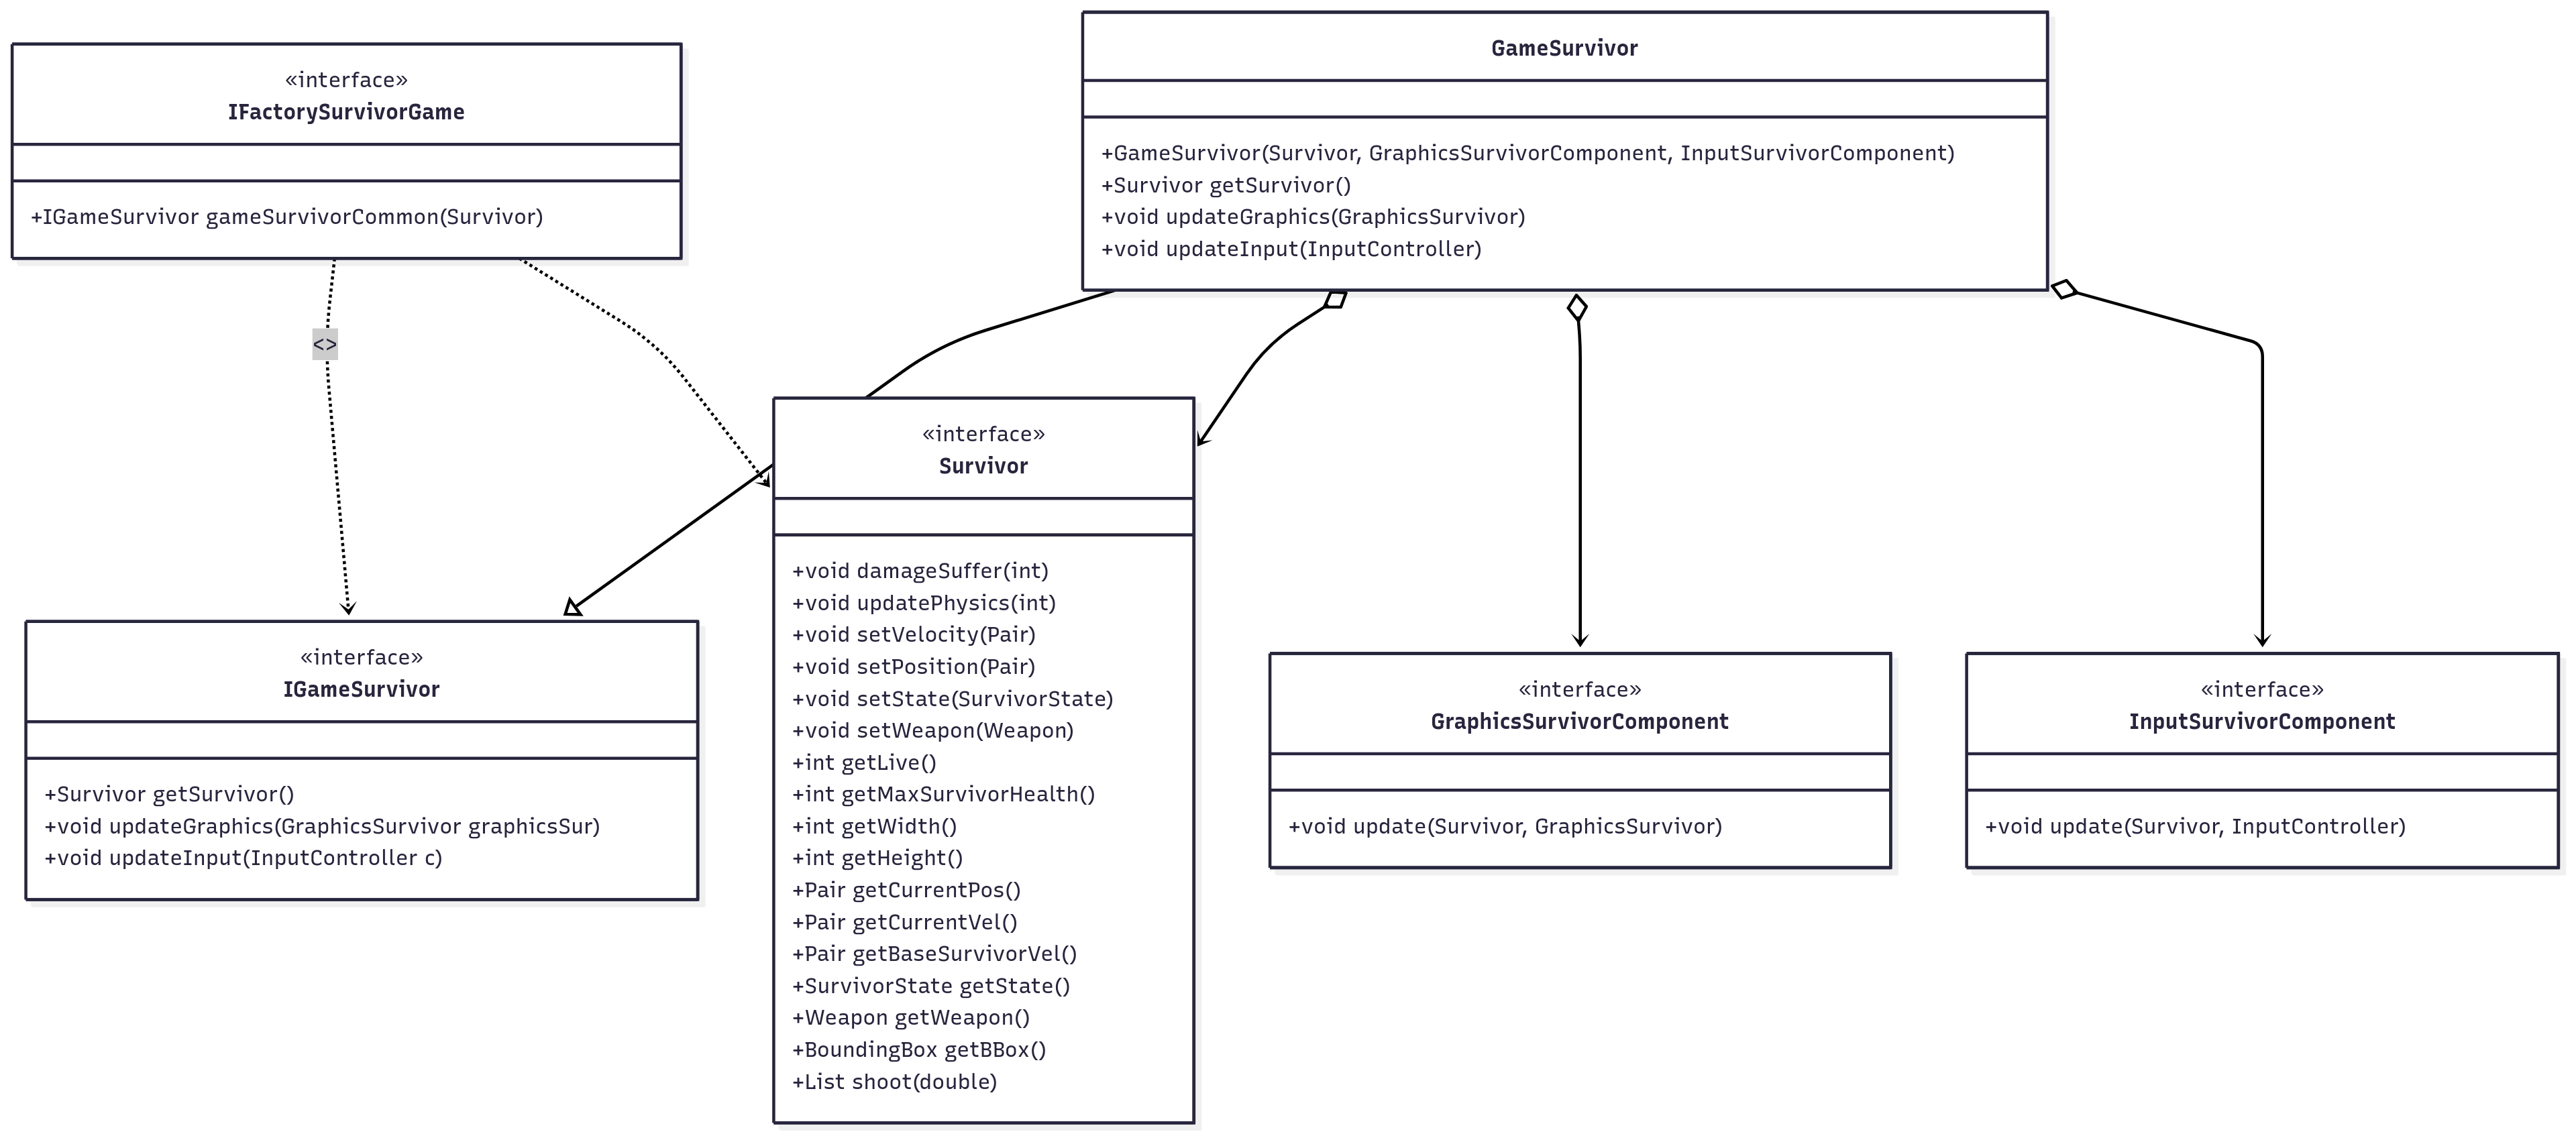
\includegraphics[width=1.0\textwidth]{img/SurvivorGame.png}
\end{center}



%%%%%%%%%%%%%%%%%%%%%%%%%%%%%%%%%%%%%%%%%%%
\section{Gestione del Survivor e uso avanzato della Factory}

In questa sezione approfondisco la gestione del \texttt{Survivor} all'interno del \texttt{package model}, con particolare attenzione all'uso della \textbf{Factory} per la sua creazione.

Il concetto fondamentale alla base di questa implementazione è che, attraverso la \texttt{SurvivorFactory}, posso costruire diversi tipi di survivor (e in modo analogo anche gli zombie, livelli o nell'armamentario vari tipi di munizioni, caricatori o Armi) assegnando loro caratteristiche ben definite fin dalla fase di istanziazione. Questo approccio rispetta il principio di separazione delle responsabilità e migliora l’estensibilità del sistema.

La factory, infatti, non si limita a creare oggetti, ma incapsula tutta la logica necessaria per configurare completamente un'entità nel mondo logico. Tra le caratteristiche configurabili tramite la factory troviamo:

\begin{itemize}
    \item \textbf{La componente fisica}: ogni survivor può essere associato a un differente comportamento fisico, implementato tramite una specifica classe del \texttt{package model.physics}. In questo modo è possibile modificare, ad esempio, la logica di movimento dell'entità senza intervenire direttamente sulla logica della classe \texttt{Survivor}.
    
    \item \textbf{Il bounding box}: la factory consente anche di specificare il tipo di \texttt{BoundingBox} da assegnare all'entità, implementato attraverso una classe del \texttt{package model.bounding\_box}. Questo permette di gestire in maniera flessibile il rilevamento delle collisioni, rendendo possibile modellare entità con forme e dimensioni differenti a seconda delle esigenze del gioco.
\end{itemize}


Questo approccio orientato ai pattern consente di centralizzare e uniformare la creazione delle entità, rendendo il codice più leggibile, manutenibile e pronto ad accogliere nuove funzionalità con un impatto minimo sul resto del sistema.

Nella pratica, l'interfaccia \texttt{ISurvivorFactory} definisce il metodo per creare i survivor, mentre la classe \texttt{SurvivorFactory} ne fornisce una concreta implementazione, specificando valori predefiniti come salute, velocità, dimensioni, fisica e bounding box. Eventuali nuovi tipi di survivor potranno essere creati facilmente estendendo la factory o aggiungendo nuove strategie di configurazione.

\begin{center}
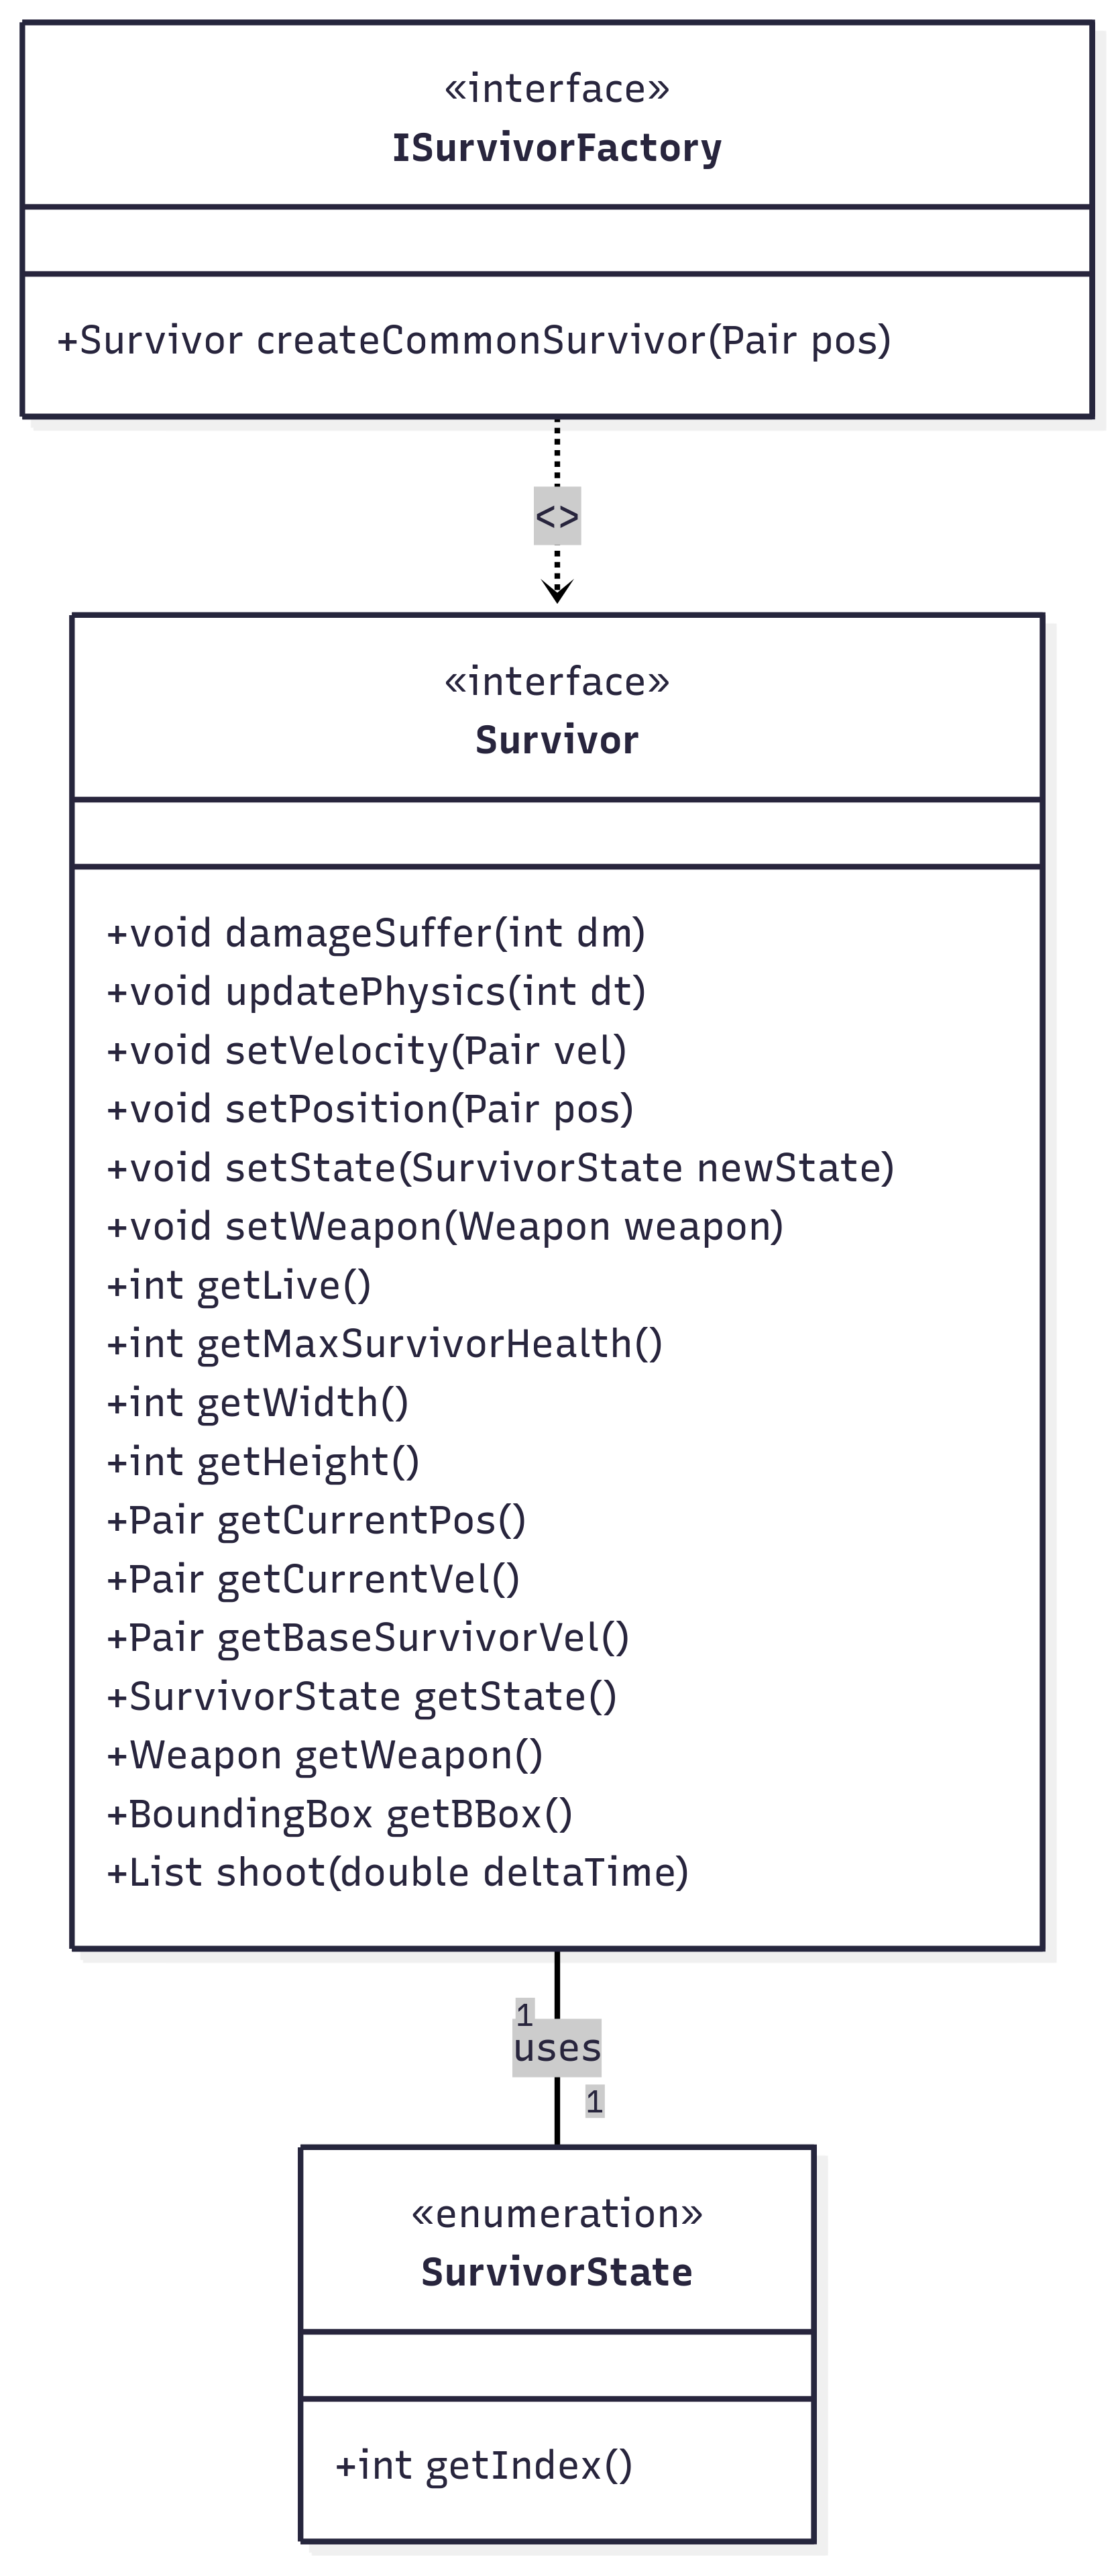
\includegraphics[width=0.3\textwidth]{img/Survivor.png}
\end{center}

\section{Gestione del Livello nel Modello}

La logica del livello di gioco è stata progettata per essere parte integrante del \texttt{model}, mantenendo una netta separazione tra le responsabilità di rappresentazione logica del mondo e quelle relative al gameplay e all'interfaccia utente. A tal fine, è stata definita un'interfaccia \texttt{Level}, implementata dalla classe concreta \texttt{LevelTutorial}, pensata come esempio base di un possibile livello.

Per supportare la creazione di diversi tipi di livelli, è stata inoltre introdotta una \textbf{factory dei livelli}, incaricata di istanziare i vari oggetti di tipo \texttt{Level} in base alle caratteristiche desiderate (es. dimensioni, bounding box e fisica).

\bigskip

Una particolarità rilevante della progettazione è l’inclusione, all’interno di ciascun \texttt{Level}, di un campo \texttt{LevelManager}. Questo componente ha un ruolo fondamentale nella gestione dinamica degli eventi di gioco interni al livello, tra cui:

\begin{itemize}
    \item \textbf{Gestione dello spawn del Survivor}: quando il livello viene avviato, il \texttt{LevelManager} si occupa di posizionare il survivor in una posizione predefinita all'interno dello scenario.
    
    \item \textbf{Controllo sullo stato del Survivor}: ad esempio per verificare se è in fase di attacco o meno.
    
    \item \textbf{Gestione dell'apparizione degli Zombie}: vengono gestite ondate (\textit{waves}) di zombie, che possono comparire a intervalli regolari. Il manager decide quante entità generare e in quali posizioni del livello (interne o esterne).
    
    \item \textbf{Creazione di zombie specifici per il livello}: ogni livello dispone del proprio \texttt{LevelManager}, che incapsula una logica personalizzata per la creazione di zombie. Questo permette di generare tipologie di nemici differenti in base al contesto, favorendo così la varietà di gameplay tra i diversi livelli.
\end{itemize}

\bigskip

Dal punto di vista strutturale, la classe \texttt{Level} contiene:

\begin{itemize}
    \item Il \texttt{Survivor} attualmente presente nel livello.
    \item Una lista di \texttt{Zombie}, attivi e visibili sulla mappa.
    \item Una lista di \texttt{Munition}, ovvero i proiettili generati nel livello durante gli scontri.
    \item Informazioni dimensionali del livello (larghezza e altezza in centimetri).
    \item Un flag che indica se il livello è completo o meno.
\end{itemize}

Il cuore della logica di aggiornamento è rappresentato dal metodo \texttt{updateLevelState}, chiamato ciclicamente nel gioco. Questo metodo è responsabile dell’evoluzione dello stato del livello: aggiornamento delle entità presenti, generazione di nuovi nemici, ecc.

\bigskip
%%%%%%%%%%%%%%%%%%%%%%%%%%%%%%%%%%%%%%%%%
\begin{center}
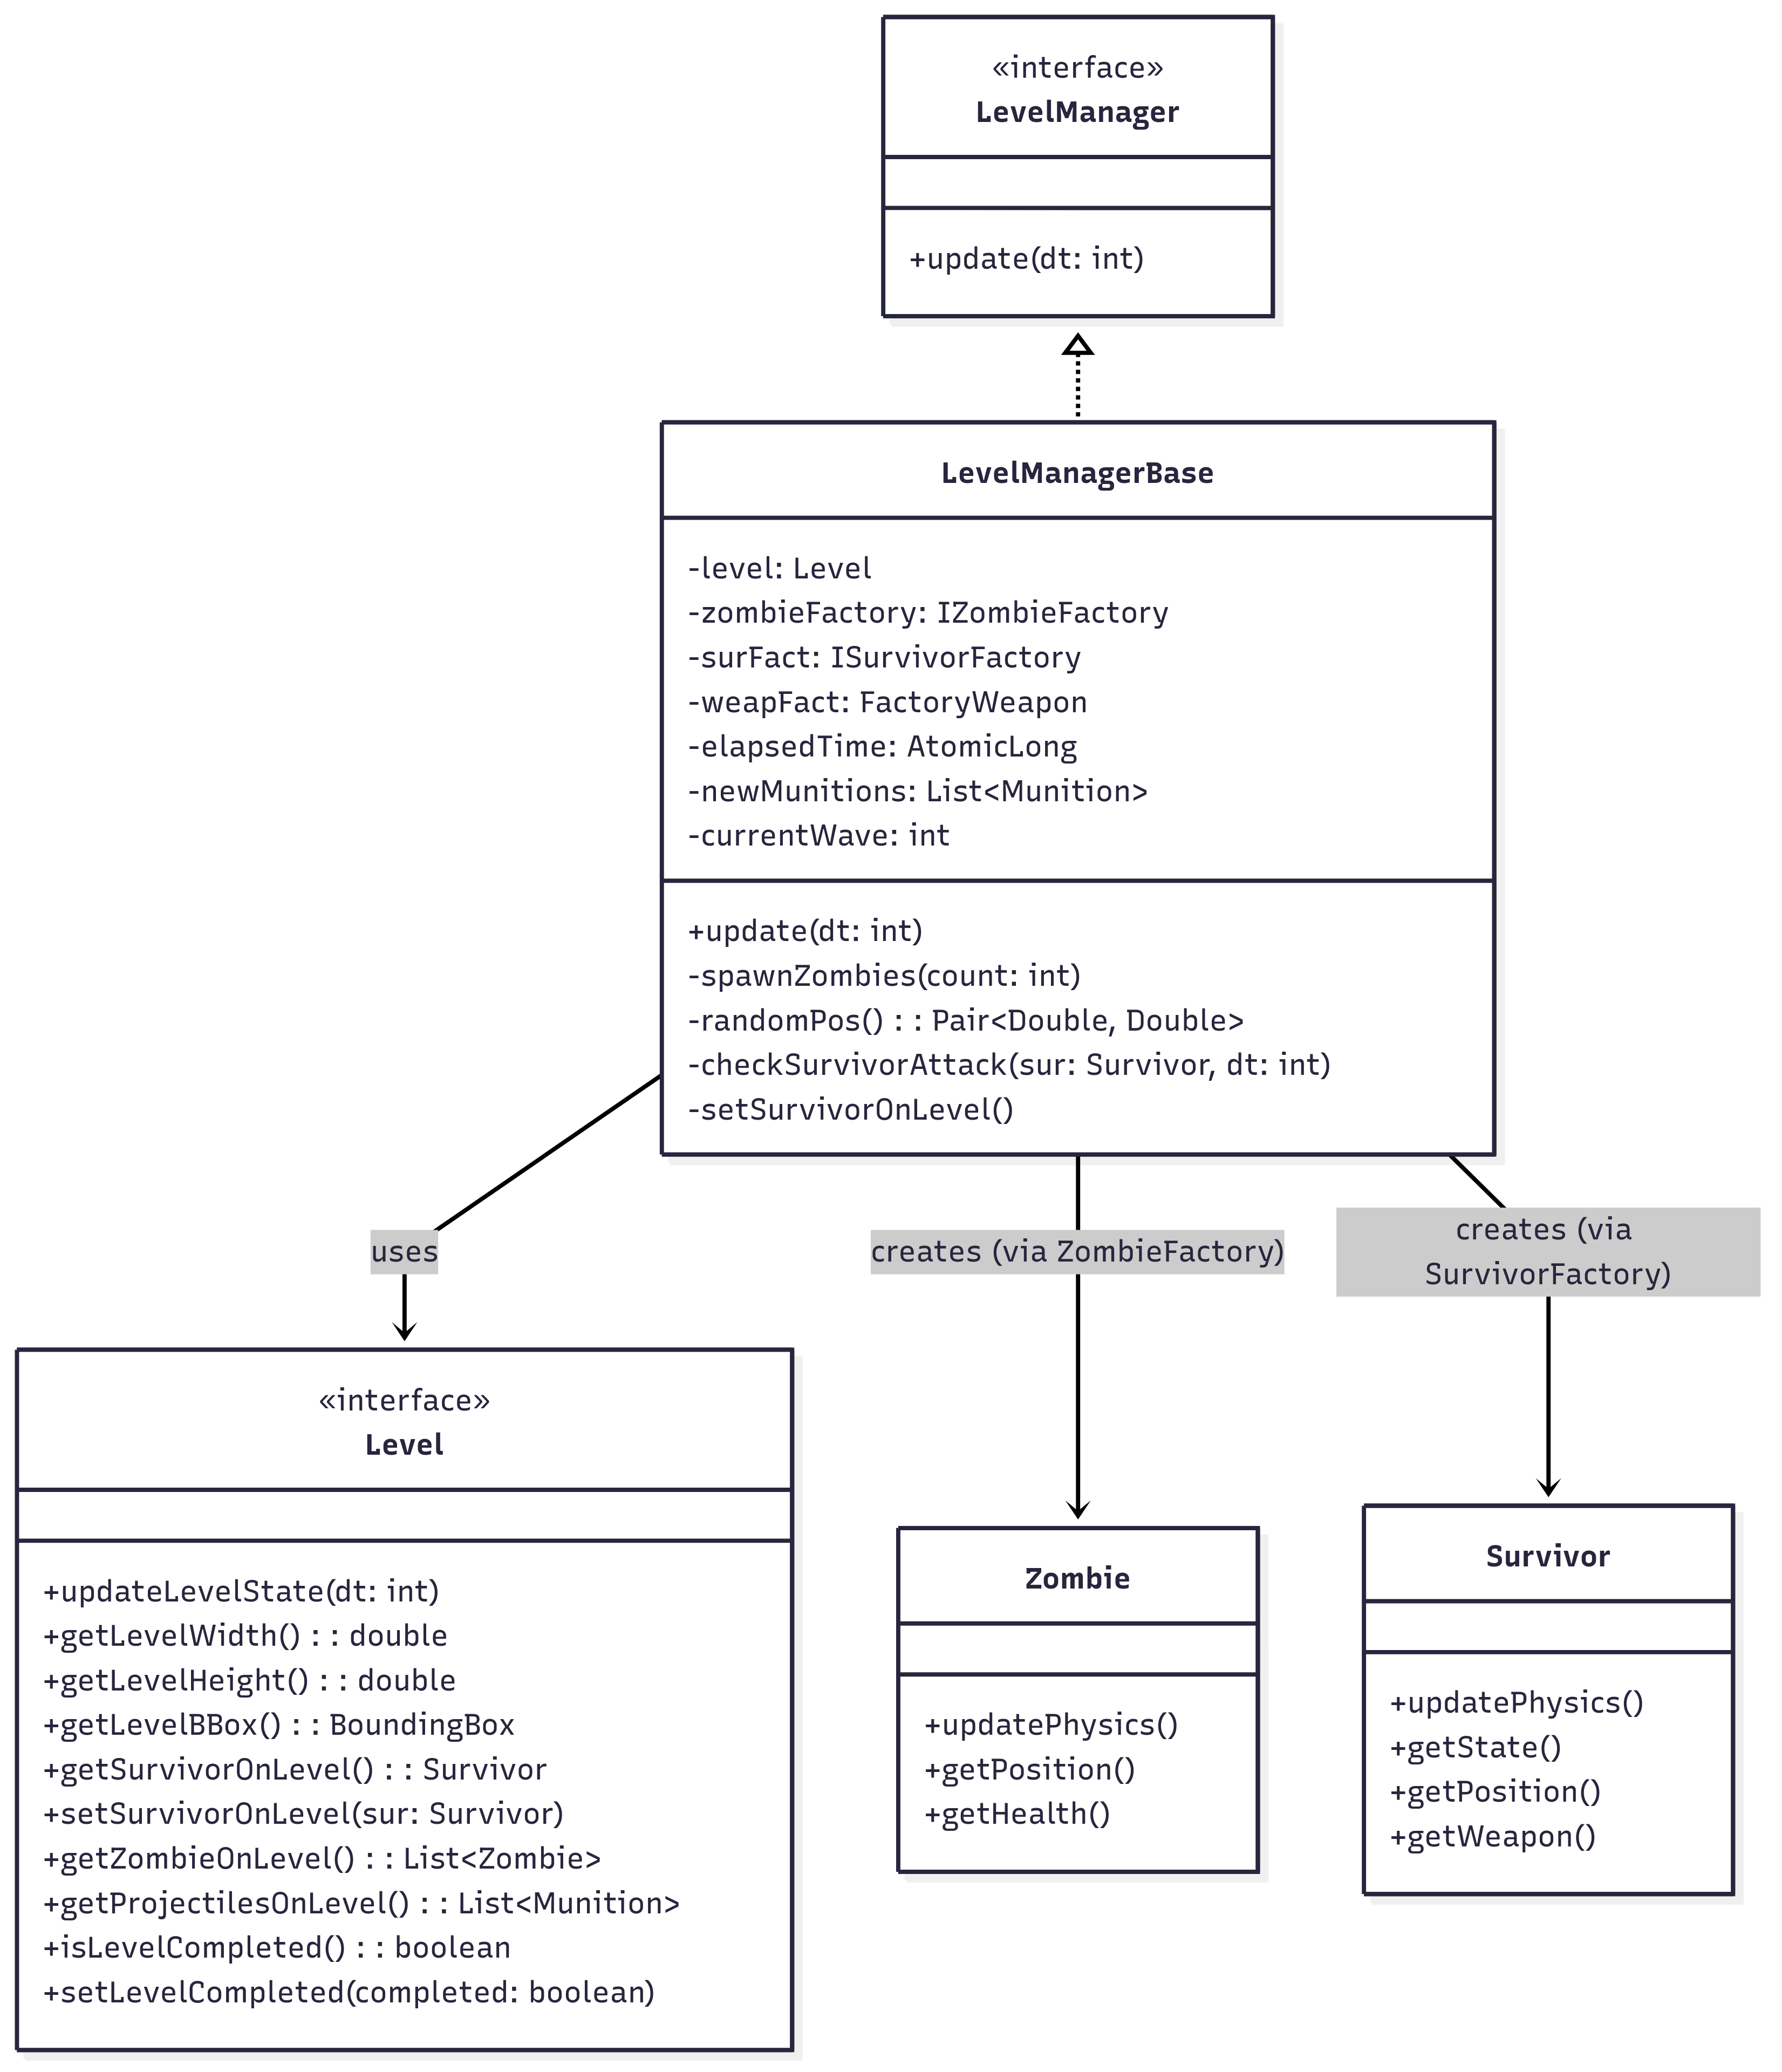
\includegraphics[width=0.5\textwidth]{img/LevelManager.png}
\end{center}
\section{Fisica del Livello e Gestione del Comportamento degli NPC}

La \textbf{componente fisica} rappresenta una parte fondamentale dell'architettura del livello, poiché si occupa della gestione della fisica di tutte le entità presenti al suo interno. In questo contesto, il termine "fisica" non si riferisce esclusivamente alla simulazione realistica delle leggi fisiche, ma alla logica che regola il movimento, le collisioni e le interazioni spaziali tra le entità di gioco.

In particolare, la fisica del livello gestisce:

\begin{itemize}
    \item \textbf{Il movimento del Survivor}: aggiornando la sua posizione in base all'input ricevuto e assicurandosi che resti sempre all'interno dei limiti del livello.
    
    \item \textbf{Il comportamento delle munizioni}: ogni proiettile sparato dal Survivor è soggetto a un sistema fisico che ne aggiorna posizione e traiettoria in base alla direzione di fuoco.
    
    \item \textbf{Il sistema di collisioni}: la componente fisica contiene anche la logica per il rilevamento e la gestione delle collisioni tra gli oggetti del gioco, come proiettili e zombie. Questo avviene tramite l'uso dei \texttt{BoundingBox} assegnati a ogni entità, i quali vengono aggiornati ad ogni frame per verificare eventuali intersezioni.
    
    \item \textbf{Il rispetto dei vincoli spaziali}: il Survivor non può uscire dai confini prestabiliti del livello, e tale vincolo è imposto proprio dalla logica fisica associata al livello stesso.
\end{itemize}

\bigskip

Un aspetto particolarmente rilevante della fisica del livello è la presenza di un campo dedicato alla gestione del comportamento dei personaggi non giocanti (NPC), ovvero gli Zombie. Questo campo è un'istanza dell'interfaccia \texttt{AINPCBehavior}, la quale definisce il comportamento di movimento degli NPC all'interno del livello.

L’oggetto \texttt{AINPCBehavior} viene generato dinamicamente tramite una \texttt{FactoryAINPCBehavior}, secondo il principio di separazione delle responsabilità e dell’inversione del controllo. Questo approccio permette di assegnare in modo modulare e flessibile una logica di movimento diversa a seconda del tipo di Zombie o delle esigenze del livello.

In fase di aggiornamento del livello, ogni Zombie invoca il comportamento definito da \texttt{AINPCBehavior}, il quale calcola la direzione ottimale verso il target, cioè il Survivor, e ne aggiorna di conseguenza la posizione. Questo sistema consente di ottenere un movimento realistico e credibile degli Zombie, che sembrano “inseguire” attivamente il giocatore, aumentando così la profondità tattica e l’immersione nel gameplay.

\bigskip
In sintesi, la componente fisica del livello agisce come un \textit{motore interno} che garantisce la coerenza e l’interattività del mondo di gioco, orchestrando il comportamento e le interazioni tra tutte le entità attive in modo modulare e facilmente estendibile.
%%%%%%%%%%%%%%%%%%%%%%%%%%%%%%%%%%%%%%%%%%%%%%%%%%%%%%%%%%%%%
\section{Approfondimento sul Comportamento degli Zombie: Strategia Composita in \texttt{AIZombieBehavior}}

A completamento della descrizione relativa al comportamento degli NPC, è opportuno analizzare più nel dettaglio il sistema che governa l'intelligenza artificiale degli \texttt{Zombie}, ovvero l'implementazione concreta dell’interfaccia \texttt{AINPCBehavior}.

Nel mio progetto, la creazione del comportamento di base per gli NPC avviene tramite un metodo della factory chiamato \texttt{createBaseNPCBehavior()}, il quale restituisce un’istanza della classe \texttt{AIZombieBehavior}. Quest’ultima rappresenta una strategia composita, costruita unendo tre comportamenti distinti ma strettamente correlati, ognuno dei quali incapsula una logica fondamentale per garantire un'interazione credibile degli zombie all’interno del livello.

In particolare, \texttt{AIZombieBehavior} è configurata con i seguenti tre componenti principali:

\begin{itemize}
    \item \textbf{Componente di movimento verso il target}: si occupa della logica di inseguimento del \texttt{Survivor}. Gli zombie calcolano la direzione ottimale in base alla posizione del giocatore e aggiornano la propria traiettoria di conseguenza, garantendo un comportamento dinamico e reattivo.

    \item \textbf{Componente di separazione (separation)}: implementa un meccanismo di “distanziamento” tra gli zombie. Quando due o più entità si trovano a una distanza minima predefinita, questa strategia regola la loro velocità o modifica leggermente la direzione di movimento, impedendo la sovrapposizione e mantenendo un comportamento collettivo realistico. Questo approccio si ispira a tecniche utilizzate nei sistemi di boid e flocking.

    \item \textbf{Componente di gestione delle collisioni tra gruppi di zombie}: interviene quando più zombie entrano in contatto diretto. In questo caso, viene applicata una logica di risoluzione delle collisioni che impedisce comportamenti incoerenti (come il completo blocco o la sovrapposizione visiva), mantenendo una corretta fisicità e interazione tra i personaggi non giocanti.
\end{itemize}

Tutte queste strategie sono iniettate all’interno dell’istanza di \texttt{AIZombieBehavior} tramite la factory. In tal modo, il comportamento dell’NPC non è rigido o codificato staticamente, ma altamente modulare e riutilizzabile. Questo design favorisce la flessibilità, poiché è possibile creare rapidamente nuove combinazioni comportamentali semplicemente sostituendo una o più delle strategie componenti, senza alterare la struttura generale del codice.

\bigskip

Questo approccio, che unisce il pattern Factory e il principio di composizione, si è rivelato estremamente efficace nella gestione dell'intelligenza artificiale nemica. Non solo ha permesso di ottenere comportamenti diversificati e realistici da parte degli zombie, ma ha anche semplificato notevolmente l'estensione futura del progetto, rendendo possibile l'introduzione di nuove tipologie di NPC dotati di logiche comportamentali alternative, come movimenti erratici, attacchi coordinati o reazioni ambientali.

\bigskip

\begin{center}
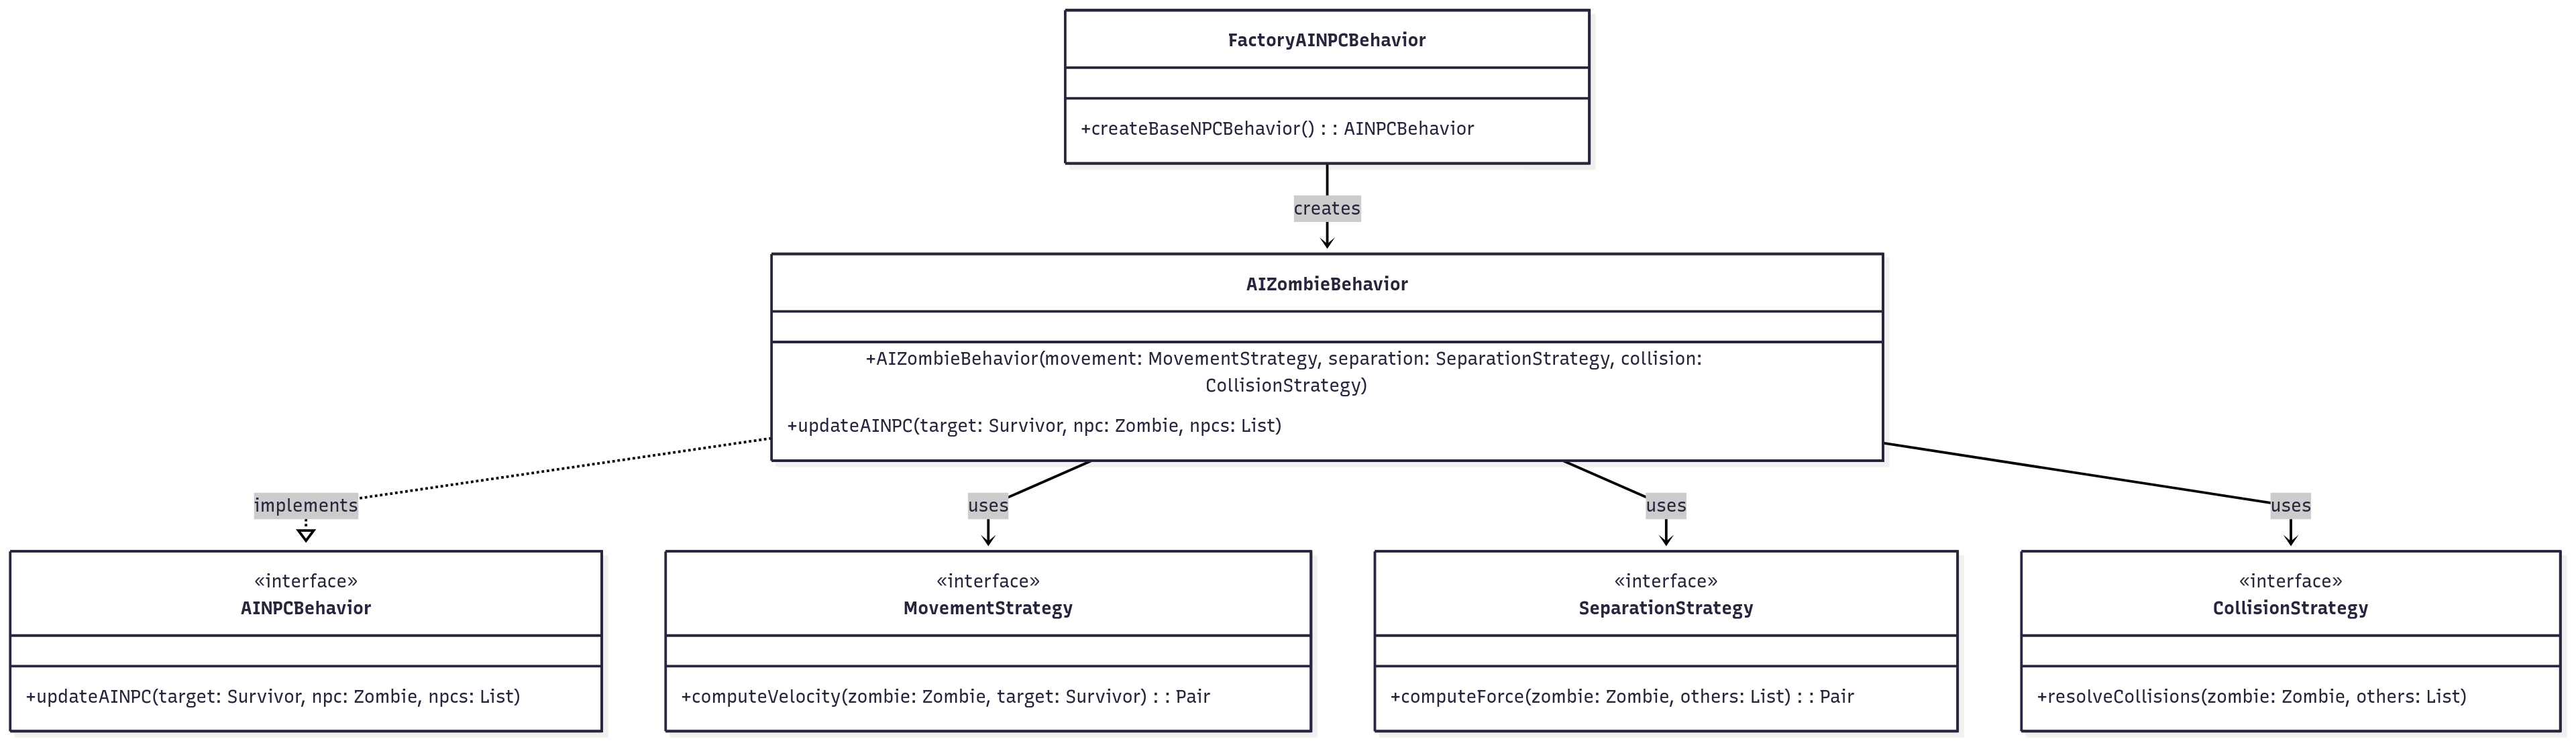
\includegraphics[width=1.0\textwidth]{img/NPCBehavior.png}
\end{center}
%%%%%%%%%%%%%%%%%%%%
\chapter{View e Gestione Grafica}

\section{Architettura della View nel Pattern MVC}

Passiamo ora alla \textbf{View}, una delle componenti più complesse del progetto a causa della necessità di rispettare il pattern MVC e garantire una netta separazione tra la logica di gioco (\textit{Model}) e la rappresentazione grafica.
Per capirla al meglio prendiamo in esempio come ho gestito la grafica del Survivor.
Nel progetto, la \texttt{GameSurvivor} svolge un ruolo centrale nella gestione della View. Per usare un’analogia artistica, può essere intesa come la \emph{tela} su cui si disegnano tutte le componenti visive relative al Survivor. Essa incapsula la logica per la visualizzazione del personaggio nel contesto di gioco, mantenendo così isolata la parte grafica dai dettagli interni del modello.

All’interno di \texttt{GameSurvivor} troviamo la \texttt{GraphicsSurvivorComponent}, la componente grafica dedicata alla rappresentazione visiva del Survivor. Questa classe si occupa di:

\begin{itemize}
    \item Gestire la \textbf{sprite sheet}, ovvero l’insieme delle immagini che compongono le diverse pose e animazioni del personaggio.
    \item Controllare l’\textbf{aggiornamento delle animazioni}, effettuando l’update dei frame per ottenere una rappresentazione fluida e dinamica del movimento e delle azioni del Survivor.
    \item Coordinare la resa grafica, che in termini artistici rappresenta la definizione dei \emph{colori}, delle forme e delle transizioni visive necessarie per mostrare lo stato attuale del personaggio.
\end{itemize}

Il metodo fondamentale di questa componente è \texttt{update}, che riceve come parametri un oggetto \texttt{Survivor} (ovvero il soggetto da disegnare, o la “modella” in termini artistici) e un’istanza di \texttt{GraphicsSurvivor}. Quest’ultima classe definisce lo \textbf{stile di disegno} e può essere implementata utilizzando diverse librerie grafiche Java, come \texttt{Java Swing} o \texttt{JavaFX}. In termini artistici, \texttt{GraphicsSurvivor} rappresenta la \emph{tecnica pittorica} o il \emph{medium} con cui la tela viene decorata, permettendo quindi di scegliere l’approccio grafico più adatto alle esigenze del progetto o alle preferenze di implementazione.

Questa suddivisione tra componente grafica e stile di disegno permette di mantenere una forte modularità e flessibilità nella gestione della View, facilitando l’estensione o la modifica delle tecniche di rendering senza impattare sulla logica del modello o del gioco.
%%%%%%%%%%%%%%%%%%%%%%%%%%%%%%%%%%%%%%%%%%%%%%%%%%%%%%%%%%%%%%%%%%%%%%%%%%%%%
\subsection{Unità di misura logica e scalatura grafica}

Un aspetto fondamentale del progetto è l'utilizzo di un'unità di misura logica uniforme per tutto il modello: il centimetro (cm). Tutti gli elementi del gioco, come l'altezza e la larghezza del \textit{Survivor}, dello \textit{Zombie}, dei proiettili, così come le dimensioni del livello stesso, sono espressi in centimetri. Questo consente una modellazione coerente e realistica dello spazio di gioco.

Tuttavia, per poter visualizzare correttamente questo mondo logico nella \textit{View}, è necessario adattare queste misure al contesto grafico. In particolare, la classe \texttt{SwingGraphicsSurvivor}, responsabile del disegno del \textit{Survivor} utilizzando le librerie \textit{Java Swing}, possiede un campo chiamato \texttt{Scaler}. Quest'ultimo viene inizializzato durante la creazione della \texttt{SwingGraphicsSurvivor} all'interno della classe \texttt{SwingSceneTutorial}.

Il compito dello \texttt{Scaler} è quello di effettuare una mappatura coerente tra le dimensioni logiche espresse in centimetri e le dimensioni del pannello grafico. In questo modo, ogni elemento viene disegnato mantenendo proporzioni e posizioni corrette rispetto allo spazio di gioco. Per esempio, se il \textit{Survivor} si trova al margine destro del pannello grafico, ciò indica che si trova realmente alla fine del livello, secondo la sua dimensione logica.

Tale approccio garantisce una separazione netta tra il modello logico e la visualizzazione, nel rispetto del pattern MVC adottato.
%%%%%%%%%%%%%%%%%%%%%%%%%%
\subsection{Gestione dell'Input}

Una parte cruciale del progetto è rappresentata dal sistema di gestione degli input, fondamentale per il controllo interattivo dei personaggi all'interno del gioco. Come precedentemente descritto, ogni oggetto di tipo \texttt{GameSurvivor} è associato a una componente di input, responsabile dell'aggiornamento dello stato sulla base delle interazioni utente.

Il metodo \texttt{update} di questa componente riceve in ingresso un oggetto di tipo \texttt{InputController}, la cui responsabilità è quella di notificare gli input ricevuti e fornire i codici di input rilevati in quel ciclo di aggiornamento. Nel progetto attuale è stata implementata una classe specifica, \texttt{KeyboardInputController}, che si occupa della gestione degli input da tastiera. Tuttavia, la struttura del sistema è pensata per essere facilmente estendibile: sarà possibile, ad esempio, integrare un controller per un gamepad, mantenendo invariato il meccanismo di comunicazione con la componente di input del \texttt{GameSurvivor}.

L'istanza di \texttt{KeyboardInputController} viene passata anche alla classe \texttt{SwingSceneTutorial}, la quale ha il compito di rilevare gli eventi generati dalla tastiera attraverso il pannello Swing e notificare tali eventi al controller. In questo contesto, l'\texttt{InputController} funge da ponte tra la scena grafica e la componente di input del survivor, garantendo così una separazione logica e strutturale tra la vista e il modello, in conformità con il pattern MVC.

Questa architettura rende l'intero sistema flessibile e modulare, favorendo l'aggiunta di nuovi dispositivi di input e il riutilizzo delle componenti esistenti.
%%%%%%%%%%%%%%%%%%%%%%%%%%%%%%%%%%%%%%%%%%%%%%%%%%%%
\section{Gestione del Game Loop e Pattern State per la Gestione degli Stati di Gioco}

Nel progetto, la logica principale di esecuzione del gioco è affidata alla classe \texttt{GameEngine}, che implementa il \emph{game loop}. Questo ciclo continuo è responsabile di orchestrare in modo sincronizzato le fasi di acquisizione dell’input, aggiornamento della logica di gioco e rendering grafico, garantendo una frequenza di aggiornamento costante e una risposta fluida alle interazioni dell’utente.

Il metodo \texttt{mainLoop()} esegue iterativamente le seguenti operazioni:
\begin{itemize}
    \item \textbf{Processamento dell’input}: attraverso il \texttt{GameStateManager}, viene delegata la gestione degli input all’attuale stato di gioco.
    \item \textbf{Aggiornamento della logica di gioco}: si invoca il metodo \texttt{updateGame()}, passando il tempo trascorso dall’ultimo aggiornamento per mantenere una simulazione temporale accurata.
    \item \textbf{Rendering}: si esegue la rappresentazione grafica dello stato di gioco corrente.
    \item \textbf{Sincronizzazione del frame rate}: grazie al metodo \texttt{waitForNextFrame()}, il ciclo viene rallentato in modo da rispettare un intervallo fisso (circa 25 ms, corrispondente a circa 40 FPS).
\end{itemize}

Questa struttura assicura un flusso di esecuzione regolare, separando chiaramente le responsabilità di input, elaborazione e output visivo.

Per gestire le diverse modalità e fasi del gioco, come ad esempio la modalità di gioco attiva o la schermata di fine partita, il progetto adotta il \emph{pattern State}. Questo pattern permette di incapsulare il comportamento specifico di ogni stato in classi dedicate che implementano l’interfaccia \texttt{GameState}, la quale definisce i metodi fondamentali per la configurazione iniziale (\texttt{setUp()}), la gestione degli input (\texttt{processInput()}), l’aggiornamento della logica (\texttt{updateGame()}) e la visualizzazione (\texttt{render()}).

La classe \texttt{GameStateManager} funge da controller centrale che mantiene il riferimento allo stato attivo e delega a esso le chiamate di input, update e render. La transizione tra stati avviene tramite il metodo \texttt{setState()}, che garantisce l’inizializzazione del nuovo stato.

Tra le implementazioni principali dello stato di gioco vi è la classe \texttt{PlayState}, responsabile della gestione della modalità di gioco attiva. Essa si occupa di caricare i livelli tramite un \texttt{PlayStateManager}, processare gli input del giocatore, aggiornare la logica di gioco — inclusi il comportamento dei nemici e le condizioni di vittoria o sconfitta — e infine gestire la transizione allo stato di gioco terminato con un ritardo controllato per consentire eventuali animazioni o messaggi finali.

Lo stato \texttt{GameOverState} rappresenta invece la fase finale del gioco, in cui viene visualizzato un messaggio di conclusione, come ad esempio la vittoria di tutti i livelli o la morte del giocatore. Questo stato si limita alla visualizzazione della schermata di fine gioco e non gestisce input o aggiornamenti della logica, fungendo da schermata informativa e di attesa.

Questo approccio modulare e scalabile consente di estendere facilmente il comportamento del gioco aggiungendo nuovi stati, senza modificare la struttura generale del motore, migliorando così la manutenibilità e la chiarezza del codice.
%%%%%%%%%%%%%%%%%%%%%

\chapter{Sviluppo}

\section{Testing}

Per garantire l'affidabilità e la correttezza del sistema, è stata adottata una strategia di testing basata su test unitari automatici, realizzati principalmente con JUnit 5. L'approccio utilizzato mira a verificare il comportamento corretto di ogni singola componente, assicurandone il corretto funzionamento in condizioni ordinarie e al contempo gestendo correttamente casi limite e situazioni di errore.

\subsection{Test delle componenti di armamento}

Le classi relative all'armamento, quali \texttt{Charger}, \texttt{Munition} e \texttt{Pistol}, sono state testate approfonditamente per validarne l'inizializzazione, il corretto comportamento dinamico e le interazioni tra oggetti.

In particolare, per la classe \texttt{Charger} si è verificato che la fabbrica crei istanze non nulle e del tipo corretto, che la capacità iniziale sia rispettata e che l'estrazione delle munizioni comporti la riduzione del carico disponibile.

La classe \texttt{Munition}, nello specifico la munizione \texttt{Parabellum}, è stata testata per la corretta inizializzazione delle proprietà (danno, dimensioni, posizione), la corretta generazione della bounding box e la gestione dello stato di tiro, con particolare attenzione al movimento post-sparo e alla gestione delle condizioni non valide.

Per quanto riguarda la classe \texttt{Pistol}, i test hanno verificato il corretto conteggio delle munizioni, il rispetto del cooldown tra i colpi e il corretto comportamento anche in presenza di più proiettili per singolo sparo.

\subsection{Test delle entità e della fisica}

Sono stati realizzati test anche per le entità del gioco, quali \texttt{Survivor} e \texttt{Zombie}. Questi test verificano la corretta gestione dei danni subiti, l'aggiornamento di posizione e velocità, la modifica dello stato interno, nonché l'integrazione con armi (mockate per isolare il test dell'entità).

I test sul \texttt{Zombie} includono la verifica della posizione iniziale, la capacità di attacco, la riduzione dei punti vita in seguito a danni e la corretta transizione di stato in caso di morte.

\subsection{Test del livello di gioco}

La classe \texttt{Level} è stata sottoposta a test per confermare la corretta inizializzazione delle dimensioni e della bounding box, la presenza di almeno un sopravvissuto e di una lista non vuota di zombie all'avvio, la corretta gestione delle liste di proiettili e la valutazione dello stato di completamento del livello in relazione alla progressione delle ondate nemiche.

\subsection{Test delle componenti grafiche e di collisione}

Infine, la classe \texttt{BoundingBox} è stata testata per validare il corretto calcolo degli angoli, la rilevazione delle collisioni (sia in presenza di sovrapposizioni che nel caso di semplici contatti sui bordi) e l'aggiornamento dinamico delle dimensioni in relazione allo spostamento dell'entità a cui è associata.

\subsection{Approccio metodologico}

L'utilizzo di framework di mocking come Mockito ha permesso di isolare i test delle entità dal comportamento delle armi, consentendo di valutare il funzionamento delle componenti singolarmente senza dipendere da implementazioni esterne. I test sono stati organizzati in modo da coprire scenari tipici, casi limite, e comportamenti attesi in presenza di input errati o stati non validi.
%%%%%%%%%%%%%%%%%%%%%%%%%%%%%%%%%%%%%%%%%%%%%%%%%%%%%%%%%%%%%%%%%%%

\chapter{Commenti finali}

\section{Autovalutazione}

Sono molto soddisfatto del lavoro svolto durante lo sviluppo del progetto, non soltanto per la quantità e qualità del codice prodotto, ma soprattutto per l'approccio adottato nella fase di progettazione. Un aspetto che ritengo particolarmente significativo è stata la ricerca e lo studio necessari per individuare e applicare correttamente i design pattern più adatti alle esigenze del progetto. In particolare, l'adozione del pattern \textit{Composite} ha rappresentato una soluzione efficace per la gestione gerarchica degli oggetti di gioco, mentre l'implementazione del pattern MVC è stata curata con attenzione per garantire una separazione chiara tra modello, vista e controllo.

Sono altresì molto soddisfatto dell'architettura sviluppata per la gestione degli input, pensata non solo per supportare gli input da tastiera, ma anche per poter essere estesa in futuro a nuovi dispositivi, come controller o touch input, senza alterare le componenti esistenti. Questo approccio riflette una visione generale di estendibilità e modularità che ha guidato l'intero progetto. L'attenzione rivolta alla futura manutenzione e all'adattabilità del codice mi ha spinto a ragionare in modo più strutturato e orientato alla progettazione software, portandomi a migliorare sensibilmente le mie competenze.

Nel complesso, considero il progetto ben riuscito sia dal punto di vista tecnico che metodologico, e rappresenta un passo significativo nel mio percorso formativo.

\subsection{Difficoltà Riscontrate}

Durante lo sviluppo del progetto, una delle principali difficoltà è stata la gestione autonoma di alcune componenti che inizialmente non rientravano nella mia assegnazione. A causa dell'assenza o dell'impossibilità di collaborazione con alcuni membri del gruppo, mi sono trovato a dover realizzare parti aggiuntive del sistema, con conseguente ridefinizione delle tempistiche e delle priorità del lavoro.

Questa situazione ha comportato un inevitabile aumento del carico di lavoro individuale e ha richiesto una riorganizzazione della pianificazione iniziale. Di conseguenza, in alcune sezioni è stato necessario procedere con soluzioni meno ottimizzate rispetto a quanto inizialmente previsto, e non è stato possibile completare pienamente tutte le funzionalità desiderate.

Nonostante ciò, l'idea progettuale di base è rimasta solida e coerente, e la struttura del progetto ha mantenuto una buona modularità. Tuttavia, l'impegno profuso per supplire ad attività non previste ha inevitabilmente influenzato la qualità e la completezza di alcune parti del codice.


\appendix
\end{document}